
%(BEGIN_QUESTION)
% Copyright 2006, Tony R. Kuphaldt, released under the Creative Commons Attribution License (v 1.0)
% This means you may do almost anything with this work of mine, so long as you give me proper credit

Følgende lagertank inneholder en væske med tetthet 60 lb/ft$^{3}$.  $\Delta$P-transmitteren er plassert 5 fot over tankbunnen og har fjernforsegling med kapillarrør der fyllevæsken har spesifikk vekt 1.9.  Ønsket nivåmåleområde er 0 fot til 11 fot:

$$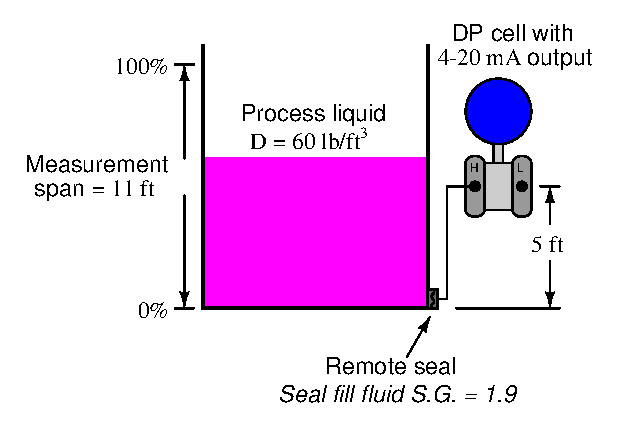
\includegraphics[width=15.5cm]{i00261x01.eps}$$

Anta en elektronisk transmitter med utgangsområde 4 til 20 mA, og kalibreringsnøyaktighet $\pm$ 0.2\% av spenn.  Fyll ut følgende kalibreringstabell:

% No blank lines allowed between lines of an \halign structure!
% I use comments (%) instead, so that TeX doesn't choke.

$$\vbox{\offinterlineskip
\halign{\strut
\vrule \quad\hfil # \ \hfil & 
\vrule \quad\hfil # \ \hfil & 
\vrule \quad\hfil # \ \hfil & 
\vrule \quad\hfil # \ \hfil & 
\vrule \quad\hfil # \ \hfil & 
\vrule \quad\hfil # \ \hfil \vrule \cr
\noalign{\hrule}
%
% First row
Prosess- & Prosent av & $\Delta$ trykk & Utgangssignal & Utgangssignal & Utgangssignal \cr
%
% Another row
nivå (ft) & spenn (\%) & målt ("W.C) & ideelt (mA) & min. (mA) & maks. (mA) \cr
%
\noalign{\hrule}
%
% Another row
  & 0 &  &  &  &  \cr
%
\noalign{\hrule}
%
% Another row
  & 10 &  &  &  &  \cr
%
\noalign{\hrule}
%
% Another row
  & 25 &  &  &  &  \cr
%
\noalign{\hrule}
%
% Another row
  & 50 &  &  &  &  \cr
%
\noalign{\hrule}
%
% Another row
  & 75 &  &  &  &  \cr
%
\noalign{\hrule}
%
% Another row
  & 90 &  &  &  &  \cr
%
\noalign{\hrule}
%
% Another row
  & 100 &  &  &  &  \cr
%
\noalign{\hrule}
} % End of \halign 
}$$ % End of \vbox

\vskip 10pt

Vis alt matematisk arbeid slik at instruktøren kan kontrollere den konseptuelle gyldigheten av metoden(e) dine.  En god kontroll er å verifisere at alle mellomregninger har fysisk mening.  {\bf Hvis du virkelig forstår hva du gjør, vil du kunne identifisere korrekt måleenhet for hvert mellomresultat og også vise hvor tallet gjelder i scenariet}.


\vskip 20pt \vbox{\hrule \hbox{\strut \vrule{} {\bf Forslag til sokratisk diskusjon} \vrule} \hrule}

\begin{itemize}
\item{} Demonstrer hvordan man kan {\it estimere} numeriske svar uten kalkulator.
\item{} Anta at tanken var lukket i toppen, med fjernforseglet kompenseringsben fra transmitterens ``L''-port til tanktoppen.  Hvordan ville dette endret nødvendig kalibrering?  Krever det justering i zero, span, linearitet, eller en kombinasjon?
\item{} Ved 100\% full tank: beregn trykket på en trykkmåler koblet i tankbunnen.
\item{} Ved 100\% full tank: beregn trykket på en trykkmåler koblet på kapillarrøret (ved fjernforseglingen).
\item{} Ved 100\% full tank: beregn trykket på en trykkmåler koblet på kapillarrøret (ved transmitterens ``H''-port).
\end{itemize}

\underbar{file i00261}
%(END_QUESTION)





%(BEGIN_ANSWER)

\noindent
{\bf Delvis svar:}

% No blank lines allowed between lines of an \halign structure!
% I use comments (%) instead, so that TeX doesn't choke.

$$\vbox{\offinterlineskip
\halign{\strut
\vrule \quad\hfil # \ \hfil & 
\vrule \quad\hfil # \ \hfil & 
\vrule \quad\hfil # \ \hfil & 
\vrule \quad\hfil # \ \hfil & 
\vrule \quad\hfil # \ \hfil & 
\vrule \quad\hfil # \ \hfil \vrule \cr
\noalign{\hrule}
%
% First row
Prosess- & Prosent av & $\Delta$ trykk & Utgangssignal & Utgangssignal & Utgangssignal \cr
%
% Another row
nivå (ft) & spenn (\%) & målt ("W.C) & ideelt (mA) & min. (mA) & maks. (mA) \cr
%
\noalign{\hrule}
%
% Another row
  & 0 &  &  &  &  \cr
%
\noalign{\hrule}
%
% Another row
  & 10 &  &  & 5.568 &  \cr
%
\noalign{\hrule}
%
% Another row
  & 25 & $-82.28$ &  &  &  \cr
%
\noalign{\hrule}
%
% Another row
5.5  & 50 &  &  &  &  \cr
%
\noalign{\hrule}
%
% Another row
  & 75 &  & 16 &  &  \cr
%
\noalign{\hrule}
%
% Another row
  & 90 &  &  &  &  \cr
%
\noalign{\hrule}
%
% Another row
  & 100 & +12.87 &  &  &  \cr
%
\noalign{\hrule}
} % End of \halign 
}$$ % End of \vbox

%(END_ANSWER)





%(BEGIN_NOTES)

% No blank lines allowed between lines of an \halign structure!
% I use comments (%) instead, so that TeX doesn't choke.

$$\vbox{\offinterlineskip
\halign{\strut
\vrule \quad\hfil # \ \hfil & 
\vrule \quad\hfil # \ \hfil & 
\vrule \quad\hfil # \ \hfil & 
\vrule \quad\hfil # \ \hfil & 
\vrule \quad\hfil # \ \hfil & 
\vrule \quad\hfil # \ \hfil \vrule \cr
\noalign{\hrule}
%
% First row
Prosess- & Prosent av & $\Delta$ trykk & Utgangssignal & Utgangssignal & Utgangssignal \cr
%
% Another row
nivå (ft) & spenn (\%) & målt ("W.C) & ideelt (mA) & min. (mA) & maks. (mA) \cr
%
\noalign{\hrule}
%
% Another row
0 & 0 & $-114$ & 4 & 3.968 & 4.032 \cr
%
\noalign{\hrule}
%
% Another row
1.1 & 10 & $-101.31$ & 5.6 & 5.568 & 5.632 \cr
%
\noalign{\hrule}
%
% Another row
2.75 & 25 & $-82.28$ & 8 & 7.968 & 8.032 \cr
%
\noalign{\hrule}
%
% Another row
5.5 & 50 & $-50.57$ & 12 & 11.968 & 12.032 \cr
%
\noalign{\hrule}
%
% Another row
8.25 & 75 & $-18.85$ & 16 & 15.968 & 16.032 \cr
%
\noalign{\hrule}
%
% Another row
9.9 & 90 & +0.1795 & 18.4 & 18.368 & 18.432 \cr
%
\noalign{\hrule}
%
% Another row
11 & 100 & +12.87 & 20 & 19.968 & 20.032 \cr
%
\noalign{\hrule}
} % End of \halign 
}$$ % End of \vbox

%INDEX% Calibration: table, level transmitter
%INDEX% Measurement, level: calibration table
%INDEX% Measurement, level: hydrostatic pressure (elevated zero)

%(END_NOTES)
